\documentclass{beamer}
\usepackage[latin1]{inputenc}
\usepackage{amsmath}
\usepackage{pgf}
\usepackage{tikz}
\usetikzlibrary{shapes}
\usepackage{PGFTikzGraph}
\usepackage{float}					% Floating figure placement.
\usepackage{graphicx}

\renewcommand\mathfamilydefault{\rmdefault}	% Math font for equations.
\usetheme{Warsaw}

% ########## Theme modifications ######################################
\usecolortheme{beaver}

% Title background
\setbeamercolor{titlelike}{parent=structure,bg=bg=gray!5!white}

% Top-right palette containing sub-sections list
\setbeamercolor*{palette primary}{fg=darkred!60!black,bg=gray!30!white}
% Top-left palette containing sections list
\setbeamercolor*{palette quaternary}{fg=white,bg=black!15!darkred}

% Bullets and enumeration style/colour
\setbeamertemplate{itemize items}[default]
\setbeamertemplate{itemize subsitem}[default]
\setbeamertemplate{enumerate items}[default]
\setbeamertemplate{enumerate subitems}[default]
\setbeamercolor{itemize item}{fg=darkred}
\setbeamercolor{itemize subitem}{fg=darkred}
\setbeamercolor{enumerate item}{fg=darkred}
\setbeamercolor{enumerate subitem}{fg=darkred}
% #####################################################################

\title{FDTD Modelling of Metamaterials Using GPU}
\author{Attique Dawood}
\institute{FAST, Islamabad}
\date{\today}
\begin{document}

\begin{frame}
\titlepage
\end{frame}

%\tableofcontents

% Introductory slide or table of contents.
\section{Organization}
\begin{frame}{Organization}
	\begin{itemize}
	\item Introduction
	\item The Finite Difference Time--Domain Technique
	\item FDTD Modelling of Metamaterials
	\item GPU Implementation of 1D and 2D DNG Slab Problems
	\item FDTD Modelling of Cylindrical Cloak
	\item Conclusion
	\end{itemize}
\end{frame}

% First slide in the introduction.
\section{Introduction}
\subsection{Computational Electromagnetics}
\begin{frame}{Computational Electromagnetics}
	\begin{itemize}
	\item Electromagnetic problems can be solved using analytical or numerical techniques
	\item Analytical methods are accurate but solution may not exist for every problem
	\item Numerical methods must be used for problems involving complex geometries
	\item Two categories of numerical methods
	\begin{enumerate}
		\item Integral (Method of Moment, Finite Element Method)
		\item Differential (Finite Difference Time--Domain)
	\end{enumerate}
	\end{itemize}
\end{frame}
\subsection{Metamaterials}
\begin{frame}{Metamaterials}
	\begin{itemize}
	\item Metamaterial concept originally put forward by Victor Veselago in the late 60's \cite{Newelectronics-Metamaterial}
	\item Metamaterials are substances with negative permittivity and permeability
	\item Artificially manufactured
	\item Behaviour can change with frequency
	\item Applications are perfect lens, invisibility cloak and novel antenna designs
	\end{itemize}
\end{frame}
\subsection{GPU Acceleration of FDTD}
\begin{frame}{GPU Acceleration of FDTD}
	\begin{itemize}
	\item FDTD requires the whole problem space to be discretised and stored in memory
	\item Availability of cheap memory 
	\item Readily paralleliseable on modern hardware involving multiple processors
	\item Modern day GPUs (Graphics Processors) are much faster than CPUs )typically 5--50 times)
	\item GPU implementation of FDTD can be much faster than CPU implementation
	\item Use GPU accelerated FDTD to model a complex problem like cylindrical cloak
	\end{itemize}
\end{frame}

% Implementation Details
\section{The Finite Difference Time--Domain Technique}
\subsection{The Yee Algorithm}
\begin{frame}{The Yee Algorithm}
	\begin{itemize}
	\item The original algorithm was proposed by K. S. Yee in 1966~\cite{Yee1966}
	\item The derivatives in Faraday's Law and Ampere's Law are replaced with difference equations
	\item Problem space is discretised and divided into cells
	\item Electric and magnetic fields are staggered at half spatial steps in unit cell
	\item By advancing the simulation in time, future values of electric and magnetic field components are computed using past values
	\end{itemize}
\end{frame}
\subsection{FDTD Update Equations in 1D}
\begin{frame}{FDTD Update Equations in 1D}
	\begin{equation*}
	\centering
	H^{n+\frac{1}{2}}_y \left[k+\frac{1}{2}\right]=H^{n-\frac{1}{2}}_y \left[k+\frac{1}{2}\right] + \dfrac{\Delta t}{\mu \Delta x} \left( E^{n}_x \left[k\right] - E^{n}_x \left[k+1\right] \right)
	\label{Hy-1D-Simple-FDTD-Driver}
	\end{equation*}
	\begin{equation*}
	\centering
	E^{n+1}_x \left[k\right]=E^{n}_x \left[k\right] + \dfrac{\Delta t}{\epsilon \Delta x} \left( H^{n+\frac{1}{2}}_y \left[k-\frac{1}{2}\right] - H^{n+\frac{1}{2}}_y \left[k+\frac{1}{2}\right] \right)
	\label{Ex-1D-Simple-FDTD-Driver}
	\end{equation*}
\end{frame}
\subsection{1D Leap--Frog Scheme}
\begin{frame}{1D Leap--Frog Scheme}
\begin{figure}[here]
\centering
\vspace{-0.5cm}
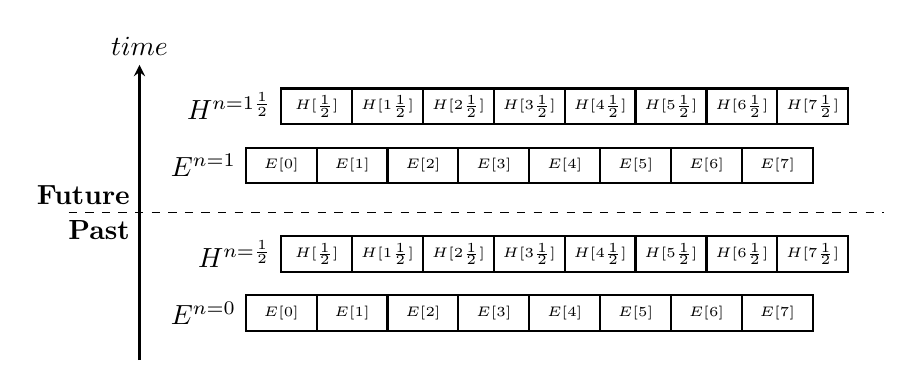
\begin{tikzpicture}[xscale=0.9,yscale=0.75]
	\def\XD{0cm}
	\def\YD{0cm}
	\coordinate[label=left:$E^{n=0}$] (E0) at (\XD,\YD+0.3cm);
	\foreach \x in {0.0cm, 1.0cm, 2.0cm, 3.0cm, 4.0cm, 5.0cm, 6.0cm, 7.0cm}
		\draw[thick] (\XD+\x, \YD+0cm) rectangle (\XD+\x+1.0cm, \YD+0.6cm);
	\foreach \x/\y in {0.0cm/0, 1.0cm/1, 2.0cm/2, 3.0cm/3, 4.0cm/4, 5.0cm/5, 6.0cm/6, 7.0cm/7}
		\draw (\XD+\x+0.5cm,\YD+0.3cm) node {{\tiny $E[\y]$}};
	
	\def\XD{0.5cm}
	\def\YD{1cm}
	\coordinate[label=left:$H^{n=\frac{1}{2}}$] (H1/2) at (\XD,\YD+0.3cm);
	\foreach \x in {0.0cm, 1.0cm, 2.0cm, 3.0cm, 4.0cm, 5.0cm, 6.0cm, 7.0cm}
		\draw[thick] (\XD+\x, \YD+0cm) rectangle (\XD+\x+1.0cm, \YD+0.6cm);
	\foreach \x/\y in {0.0cm/\frac{1}{2}, 1.0cm/1\frac{1}{2}, 2.0cm/2\frac{1}{2}, 3.0cm/3\frac{1}{2}, 4.0cm/4\frac{1}{2}, 5.0cm/5\frac{1}{2}, 6.0cm/6\frac{1}{2}, 7.0cm/7\frac{1}{2}}
		\draw (\XD+\x+0.5cm,\YD+0.3cm) node {{\tiny $H[\y]$}};

	\draw[dashed] (-2.5cm,2cm) -- (9.0cm,2cm);

	\def\XD{0cm}
	\def\YD{2.5cm}
	\coordinate[label=left:$E^{n=1}$] (E1) at (\XD,\YD+0.3cm);
	\foreach \x in {0.0cm, 1.0cm, 2.0cm, 3.0cm, 4.0cm, 5.0cm, 6.0cm, 7.0cm}
		\draw[thick] (\XD+\x, \YD+0cm) rectangle (\XD+\x+1.0cm, \YD+0.6cm);
	\foreach \x/\y in {0.0cm/0, 1.0cm/1, 2.0cm/2, 3.0cm/3, 4.0cm/4, 5.0cm/5, 6.0cm/6, 7.0cm/7}
		\draw (\XD+\x+0.5cm,\YD+0.3cm) node {{\tiny $E[\y]$}};

	\def\XD{0.5cm}
	\def\YD{3.5cm}
	\coordinate[label=left:$H^{n=1\frac{1}{2}}$] (H11/2) at (\XD,\YD+0.3cm);
	\foreach \x in {0.0cm, 1.0cm, 2.0cm, 3.0cm, 4.0cm, 5.0cm, 6.0cm, 7.0cm}
		\draw[thick] (\XD+\x, \YD+0cm) rectangle (\XD+\x+1.0cm, \YD+0.6cm);
	\foreach \x/\y in {0.0cm/\frac{1}{2}, 1.0cm/1\frac{1}{2}, 2.0cm/2\frac{1}{2}, 3.0cm/3\frac{1}{2}, 4.0cm/4\frac{1}{2}, 5.0cm/5\frac{1}{2}, 6.0cm/6\frac{1}{2}, 7.0cm/7\frac{1}{2}}
		\draw (\XD+\x+0.5cm,\YD+0.3cm) node {{\tiny $H[\y]$}};


	\draw[thick, ->, >=stealth] (-1.5cm, -0.5cm) -- (-1.5cm, 4.5cm);
	\coordinate[label=above:$time$] (time) at (-1.5cm,4.5cm);
	\coordinate[label=left:\textbf{Past}] (Past) at (-1.5cm,1.7cm);
	\coordinate[label=left:\textbf{Future}] (Future) at (-1.5cm,2.3cm);

\end{tikzpicture}
%\caption{FDTD leap--frog\index{leap--frog} scheme to update future fields from past fields}
\label{FDTD-LeapFrog}
\end{figure}
\end{frame}
\subsection{Courant Stability Criteria}
\begin{frame}{Courant Stability Criteria}
\begin{equation*}
\centering
c \Delta t \leq \left[ \dfrac{1}{\Delta x^2} + \dfrac{1}{\Delta y^2} + \dfrac{1}{\Delta z^2} \right]^{-\frac{1}{2}}
\label{Courant-Stability-Criterion}
\end{equation*}
\begin{equation*}
\centering
S_c = \dfrac{c \Delta t}{\Delta} \leq 1,~\Delta=\Delta x = \Delta y =\Delta z
\label{Courant-Stability-Criterion-Equal-Differentials}
\end{equation*}
	\begin{itemize}
	\item $S_c$ is known as Courant Number
	\item In one time step ($\Delta t$) the amount of distance travelled by an electromagnetic wave (in cells) is equal to Courant number
	\item  Smaller values of $S_c$ will result in better stability but the trade--off is an increase in simulation time
	\end{itemize}
\end{frame}
\section{FDTD Modelling of Metamaterials Using Drude Model}
\subsection{Limitations of FDTD}
\begin{frame}{Limitations of FDTD}
	\begin{itemize}
	\item In conventional FDTD material cannot be simply assigned negative (or close to 0) values of permittivity or permeability
	\item Due to Courant Stability Criteria FDTD implementation will be unstable
	\item Drude and Lorentz dispersion models give negative values of permittivity/permeability for certain frequency range
	\item Negative permittivity and permeability can be modelled using these dispersion models
	\end{itemize}
\end{frame}
\subsection{Drude Dispersion Model}
\begin{frame}{Drude Dispersion Model}
	\begin{itemize}
	\item In ideal conditions the permittivity (and permeability) of a material remain constant for any frequency and throughout the structure of that material
	\item Speed of electromagnetic waves in such a medium remain constant if frequency changes
	\item In reality, such a material does not exist
	\item Speed of EM waves varies with frequency of operation
	\end{itemize}
	\begin{equation*}
	\centering
	\hat{\epsilon_r}(\omega)=\epsilon_\infty-\dfrac{\omega^2_p}{\omega^2-jg\omega}
	\label{er-Drude}
	\end{equation*}
\end{frame}
\subsection{Drude Model Permittivity Vs Frequency}
\begin{frame}{Drude Model Permittivity Vs Frequency}
\begin{figure}[H]
\centering
\vspace{-0.35cm}
\includegraphics[scale=0.525, trim=4cm 8.5cm 4cm 8.5cm, clip]{Figures/FigCh03_DrudeModel_er.pdf}
\vspace{-0.5cm}
\caption{{\tiny $\epsilon_r$ plotted against $\omega/\omega_p$ for $\epsilon_\infty=1$ and $g=0$}}
\label{DrudeModel_er}
\end{figure}
\end{frame}
\subsection{Auxiliary Update Equations Based on Drude Model}
\begin{frame}{Auxiliary Update Equations Based on Drude Model}
\vspace{-0.5cm}
\begin{equation*}
\centering
\textbf{B} = \mu \textbf{H}
\label{B-mu-H}
\end{equation*}
\begin{equation*}
\centering
\nonumber \textbf{B} \left( \dfrac{\omega^2-jg\omega}{\mu_\infty(\omega^2-jg\omega)-\omega^2_p} \right) =\textbf{H}
\label{B-muomega-H}
\end{equation*}
\begin{eqnarray*}
\nonumber H^{n+1}_y &=& a_m\left(B^{n+1}_y-2B^n_y+B^{n-1}_y\right)+b_m\left(B^{n+1}_y-B^{n-1}_y\right)\\
&&+c_m\left(2H^n_y-H^{n-1}_y\right)+d_m\left(2H^n_y+H^{n-1}_y\right)+e_m H^{n-1}_y
\label{2nd-order-B-H-final-form}
\end{eqnarray*}
\begin{eqnarray*}
\nonumber E^{n+1}_x &=& a_e\left(D^{n+1}_x-2D^n_x+D^{n-1}_x\right)+b_e\left(D^{n+1}_x-D^{n-1}_x\right)\\
&&+c_e\left(2E^n_x-E^{n-1}_x\right)+d_e\left(2E^n_x+E^{n-1}_x\right)+e_e E^{n-1}_x
\label{2nd-order-D-E-final-form}
\end{eqnarray*}
\end{frame}
\subsection{FDTD Update Equations}
\begin{frame}{FDTD Update Equations}
For a wave propagating in $z$ direction, FDTD update equations\index{FDTD!update equations} are
\begin{equation}
B^{n+1}_y(k)=B^n_y(k)+\dfrac{\Delta t}{\Delta z}\left(E^n_x(k)-E^n_x(k+1)\right)
\label{1D-B-Update-Equation}
\end{equation}
and
\begin{equation}
D^{n+1}_x(k)=D^n_x(k)+\dfrac{\Delta t}{\Delta z}\left(H^{n+1}_y(k-1)-H^{n+1}_y(k)\right).
\label{1D-D-Update-Equation}
\end{equation}
\end{frame}
\subsection{Dispersive FDTD Algorithm}
\begin{frame}{Dispersive FDTD Algorithm}
\begin{enumerate}
\item Compute future value of $B_y$ from past values of $B_y$ and $E_x$ (equation \ref{1D-B-Update-Equation}).
\item Compute future value of $H_y$ from $B_y$ calculated in step 1 (auxiliary update equation for $H_y$).
\item Compute future value of $D_x$ from past value of $D_x$ and $H_y$ in step 2 (equation \ref{1D-D-Update-Equation}).
\item Compute future value of $E_x$ from $D_x$ calculated in step 3 (auxiliary update equation for $E_x$).
\item Update additive source at specified source location for current time step.
\end{enumerate}
\end{frame}
\section{GPU Implementation of 1D and 2D DNG Slab Problems}
\subsection{Problem Geometry}
\begin{frame}{Problem Geometry}
\begin{figure}[H]
\centering
\vspace{-0.5cm}
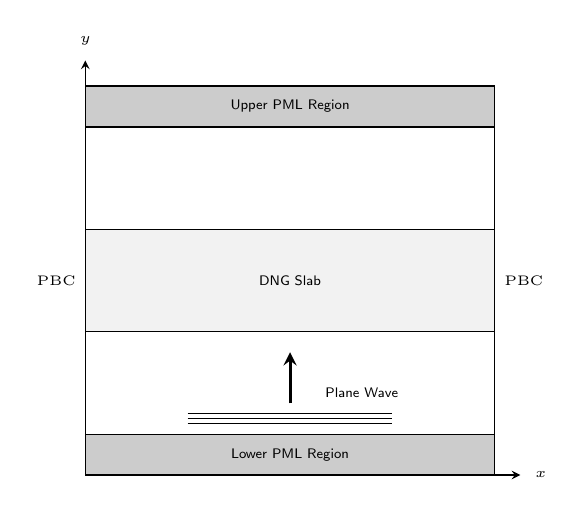
\begin{tikzpicture}[xscale=0.65,yscale=0.65]
	\newcommand{\LeftX}{0cm}
	\newcommand{\MidX}{4cm}
	\newcommand{\RightX}{8cm}
	\newcommand{\PMLw}{0.8cm}
	\newcommand{\DomainY}{6.0cm}
	\newcommand{\SlabStartY}{2.0cm+\PMLw}
	\newcommand{\SlabEndY}{4.0cm+\PMLw}
	% x-axis.
	\draw[->, >=stealth] (\LeftX,0cm) -- (\RightX+0.5cm,0cm);
	\coordinate [label=right:{\tiny $x$}] (x-axis) at (\RightX+0.6cm,0cm);
	% y-axis.
	\draw[->, >=stealth] (\LeftX,0cm) -- (\LeftX,2*\PMLw+\DomainY+0.5cm);
	\coordinate [label=above:{\tiny $y$}] (y-axis) at (\LeftX,2*\PMLw+\DomainY+0.6cm);
	% PBCs.
	\coordinate [label=right:{\tiny PBC}] (PBCright) at (\RightX,\PMLw+3.0cm);
	\coordinate [label=left:{\tiny PBC}] (PBCleft) at (\LeftX,\PMLw+3.0cm);
	% Lower PML Region.
	\draw[fill=gray!40!white] (\LeftX,0cm) rectangle (\RightX,\PMLw);
	\coordinate [label=center:{\tiny \textsf{Lower PML Region}}] (LowerPML) at (\MidX,0.4cm);
	% Solution Region.
	\draw (\LeftX,\PMLw) rectangle (\RightX,\PMLw+\DomainY);
	% Upper PML Region.
	\draw[fill=gray!40!white] (\LeftX,\PMLw+\DomainY) rectangle (\RightX,2*\PMLw+\DomainY);
	\coordinate [label=center:{\tiny \textsf{Upper PML Region}}] (UpperPML) at (\MidX,\PMLw+\DomainY+0.4cm);
	% Slab.
	\draw[fill=gray!10!white] (\LeftX,\SlabStartY) rectangle (\RightX,\SlabEndY);
	\coordinate [label=center:{\tiny \textsf{DNG Slab}}] (DNGSlab) at (\MidX,\PMLw+3.0cm);
	% Plane wave.
	\draw (\LeftX+2.0cm,\PMLw+0.2cm) -- (\RightX-2.0cm, \PMLw+0.2cm);
	\draw (\LeftX+2.0cm,\PMLw+0.3cm) -- (\RightX-2.0cm, \PMLw+0.3cm);
	\draw (\LeftX+2.0cm,\PMLw+0.4cm) -- (\RightX-2.0cm, \PMLw+0.4cm);
	\draw[line width=1.1pt, ->, >=stealth] (\MidX,\PMLw+0.6cm) -- (\MidX,\PMLw+1.6cm);
	\coordinate [label=right:{\tiny \textsf{Plane Wave}}] (PlaneWave) at (\MidX+0.5cm,\PMLw+0.8cm);
\end{tikzpicture}
\label{fig:2D-DNG-Geometry}
\end{figure}
\end{frame}
\subsection{FDTD Update Equations in 2D}
\begin{frame}{FDTD Update Equations in 2D}
FDTD update equations for the $TM^z$ case are
\begin{equation}
\begin{split}
D^{n+1}_z \left[i,j\right]=D^{n}_z \left[i,j\right]+\dfrac{\Delta t}{\Delta}&\left(H^{n+1}_y\left[i,j\right]-H^{n+1}_y \left[i-1,j\right]\right.\\
&\left.-H^{n+1}_x \left[i,j+1\right]+H^{n+1}_x \left[i,j\right]\right),
\end{split}
\label{eq:Dz-2D-FDTD-TMz-Corrected}
\end{equation}
\begin{equation}
B^{n+1}_x \left[i,j\right]=B^n_x \left[i,j\right] + \dfrac{\Delta t}{\Delta} \left(-E^{n}_z \left[i,j\right] + E^{n}_z \left[i,j-1\right] \right)
\label{eq:Bx-2D-FDTD-TMz-Corrected}
\end{equation}
and
\begin{equation}
B^{n+1}_y \left[i,j\right]=B^n_y \left[i,j\right] + \dfrac{\Delta t}{\Delta} \left( E^{n}_z \left[i+1,j\right] - E^{n}_z \left[i,j\right] \right).
\label{eq:By-2D-FDTD-TMz-Corrected}
\end{equation}
\end{frame}
\subsection{Arrangement of Field Nodes}
\begin{frame}{Arrangement of Field Nodes}
\begin{figure}[H]
\centering
\vspace{-0.4cm}
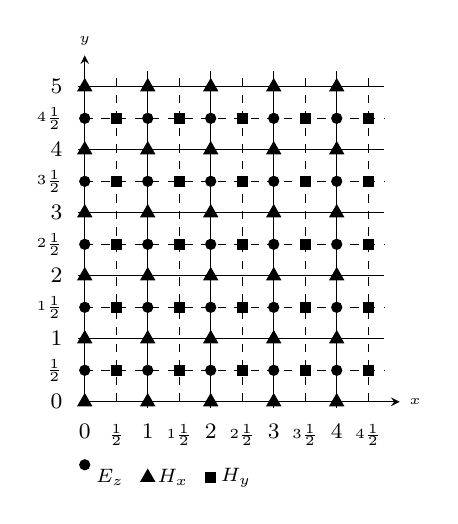
\begin{tikzpicture}[xscale=0.8,yscale=0.8]
	\newcommand{\LeftX}{0cm}
	\newcommand{\RightX}{5cm}
	\newcommand{\LowY}{0cm}
	\newcommand{\HighY}{5.5cm}
	% x-axis.
	\draw[->, >=stealth] (\LeftX,\LowY) -- (\RightX,\LowY);
	\coordinate [label=right:{\tiny $x$}] (x-axis) at (\RightX+0.0cm,\LowY);
	% y-axis.
	\draw[->, >=stealth] (\LeftX,\LowY) -- (\LeftX,\HighY);
	\coordinate [label=above:{\tiny $y$}] (y-axis) at (\LeftX,\HighY+0.0cm);
	% Drawing vertical grid lines.
	\foreach \x in {1cm,2cm,3cm,4cm}
		\draw (\x,\LowY-0.1cm) -- (\x,\HighY-0.25cm); % Solid lines at +1 intervals.
	\foreach \x in {0.5cm,1.5cm,2.5cm,3.5cm,4.5cm}
		\draw[dashed] (\x,\LowY) -- (\x,\HighY-0.25cm); % Dashed lines at 1/2 intervals.
	% Drawing horizontal grid lines.
	\foreach \y in {1cm,2cm,3cm,4cm,5cm}
		\draw (\LeftX-0.1cm,\y) -- (\RightX-0.25cm,\y); % Solid lines at +1 intervals.
	\foreach \y in {0.5cm,1.5cm,2.5cm,3.5cm,4.5cm}
		\draw[dashed] (\LeftX,\y) -- (\RightX-0.25cm,\y); % Dashed lines at 1/2 intervals.
	% Drawing nodes.
	\foreach \x in {0cm,1cm,2cm,3cm,4cm}
		\foreach \y in {0.5cm,1.5cm,2.5cm,3.5cm,4.5cm}
			\filldraw (\x,\y) circle (0.08cm); % Ez nodes.
	\foreach \x in {0.5cm,1.5cm,2.5cm,3.5cm,4.5cm}
		\foreach \y in {0.5cm,1.5cm,2.5cm,3.5cm,4.5cm}
			\node[fill=black,regular polygon, regular polygon sides=4,inner sep=0.05cm] at (\x,\y) {}; % Hy nodes.
	\foreach \x in {0cm,1cm,2cm,3cm,4cm}
		\foreach \y in {0cm,1cm,2cm,3cm,4cm,5cm}
			\node[fill=black,regular polygon, regular polygon sides=3,inner sep=0.04cm] at (\x,\y) {}; % Hx nodes.
	% +1 Text for x-axis.
	\foreach \x/\t in {0cm/0,1cm/1,2cm/2,3cm/3,4cm/4}
		\coordinate [label=below:{\footnotesize $\t$}] (\t) at (\x,\LowY-0.2cm);
	% 1/2 Text for x-axis.
	\foreach \x/\t in {0.5cm/ ,1.5cm/1,2.5cm/2,3.5cm/3,4.5cm/4}
		\coordinate [label=below:{\tiny $\t\frac{1}{2}$}] (\t) at (\x,\LowY-0.2cm);
	% +1 Text for y-axis.
	\foreach \y/\t in {0cm/0,1cm/1,2cm/2,3cm/3,4cm/4,5cm/5}
		\coordinate [label=left:{\footnotesize $\t$}] (\t) at (\LeftX-0.2cm,\y);
	% 1/2 Text for y-axis.
	\foreach \y/\t in {0.5cm/ ,1.5cm/1,2.5cm/2,3.5cm/3,4.5cm/4}
		\coordinate [label=left:{\tiny $\t\frac{1}{2}$}] (\t) at (\LeftX-0.2cm,\y);
	% Legend
	\filldraw (\LeftX+0cm,\LowY-1cm) circle (0.08cm); % Ez.
	\coordinate [label=center:{\scriptsize $E_z$}] (EzLegend) at (\LeftX+0.4cm,\LowY-1.2cm);
	\node[fill=black,regular polygon, regular polygon sides=3,inner sep=0.04cm] at (\LeftX+1cm,\LowY-1.2cm) {}; % Hx.
	\coordinate [label=center:{\scriptsize $H_x$}] (HxLegend) at (\LeftX+1.4cm,\LowY-1.2cm);
	\node[fill=black,regular polygon, regular polygon sides=4,inner sep=0.05cm] at (\LeftX+2cm,\LowY-1.2cm) {}; % Hy.
	\coordinate [label=center:{\scriptsize $H_y$}] (HxLegend) at (\LeftX+2.4cm,\LowY-1.2cm);
\end{tikzpicture}
\label{fig:2D-DNG-Field-Nodes}
\end{figure}
\end{frame}
\subsection{Simulation Parameters (2D)}
\begin{frame}{Simulation Parameters (2D)}
	\begin{itemize}
	\item Simulation size is $512\times 512$ cells
	\item PML width is 50 cells
	\item $\Delta = 3 mm$ and $\Delta t = 50 ps$ with $S_c=0.5$
	\item $f_0=1.5625 GHz$
	\item  To obtain relative permittivity and permeability of $-1$ at required $f_0$, plasma frequencies are set as $\omega^2_{pm}=\omega^2_{pe}=2\times(2\pi f_0)^2$ with $\epsilon_\infty=\mu_\infty=1$
	\end{itemize}
\end{frame}
\subsection{Refractive Index}
\begin{frame}{Refractive Index}
\begin{figure}[H]
\centering
\includegraphics[scale=0.5, trim=3.5cm 8.7cm 4.5cm 8.85cm, clip]{Figures/FigCh03_2DDNGRefractiveIndex.pdf}
%\caption{Refractive index of 2D DNG slab}
\label{fig:2DDNG-Refractive-Index}
\end{figure}
\end{frame}
\subsection{Performance Analysis}
\begin{frame}{Performance Analysis: 2D Spatial}
\begin{figure}[H]
\vspace{-0.5cm}
\centering
	\begin{tikzpicture}[xscale=0.6,yscale=0.6]
		\DrawAxes{size}{time~(sec)}
		\GridOn
		\TicksOn
		\XAxisText{0.313cm/32^2}{1.25cm/128^2}{2.5cm/256^2}{3.75cm/384^2}{ 5cm/512^2}{6.25cm/640^2}{7.5cm/768^2}{8.75cm/896^2}{10cm/1024^2}
		\YAxisText{0.00cm/0}{1.00cm/60}{2.00cm/120}{3.00cm/180}{4.00cm/240}{5.00cm/300}{6.00cm/360}{7.00cm/420}{8.00cm/480}
		\YAxisText{9.00cm/540}{10.00cm/600}{}{}{}{}{}{}{}
		% 2D spatial all plots with 256 time steps
		\draw[line width=1.2pt,color=red!40!yellow] (0.31cm,0.019cm) -- (0.63cm,0.025cm) -- (1.3cm,0.048cm) -- (2.5cm,0.2cm) -- (3.8cm,0.59cm) -- ( 5cm,1.2cm) -- (6.3cm,2.1cm) -- (7.5cm,3.3cm) -- (8.8cm,4.4cm) -- (10cm, 6cm);
		\draw[line width=1.2pt,color=red!10!yellow] (0.31cm,0.00082cm) -- (0.63cm,0.0038cm) -- (1.3cm,0.02cm) -- (2.5cm,0.3cm) -- (3.8cm,0.41cm) -- ( 5cm,2.5cm) -- (6.3cm,2.5cm) -- (7.5cm,5.2cm) -- (8.8cm,5.9cm) -- (10cm,9.8cm);
		\draw[line width=1.2pt,color=blue] (0.31cm,0.00087cm) -- (0.63cm,0.0033cm) -- (1.3cm,0.017cm) -- (2.5cm,0.32cm) -- (3.8cm,0.5cm) -- ( 5cm,2.1cm) -- (6.3cm,2.7cm) -- (7.5cm,4.4cm) -- (8.8cm,5.6cm) -- (10cm,8.5cm);
		\draw[line width=1.2pt,color=blue!30!white] (0.31cm,0.0032cm) -- (0.63cm,0.0062cm) -- (1.3cm,0.022cm) -- (2.5cm,0.13cm) -- (3.8cm,0.37cm) -- ( 5cm,2.3cm) -- (6.3cm,2.3cm) -- (7.5cm,4.8cm) -- (8.8cm,5.4cm) -- (10cm,9.2cm);
		\draw[line width=1.2pt,color=gray!70!white] (0.31cm,0.0093cm) -- (0.63cm,0.011cm) -- (1.3cm,0.017cm) -- (2.5cm,0.049cm) -- (3.8cm,0.091cm) -- ( 5cm,0.17cm) -- (6.3cm,0.24cm) -- (7.5cm,0.36cm) -- (8.8cm,0.5cm) -- (10cm,0.66cm);
		\draw[line width=1.2pt,color=pink] (0.31cm,0.013cm) -- (0.63cm,0.013cm) -- (1.3cm,0.017cm) -- (2.5cm,0.046cm) -- (3.8cm,0.095cm) -- ( 5cm,0.18cm) -- (6.3cm,0.25cm) -- (7.5cm,0.36cm) -- (8.8cm,0.45cm) -- (10cm,0.66cm);
		\draw[line width=1.2pt,color=red!70!black] (0.31cm,0.0022cm) -- (0.63cm,0.0027cm) -- (1.3cm,0.0035cm) -- (2.5cm,0.0078cm) -- (3.8cm,0.014cm) -- ( 5cm,0.023cm) -- (6.3cm,0.034cm) -- (7.5cm,0.049cm) -- (8.8cm,0.066cm) -- (10cm,0.085cm);
		\draw[line width=1.2pt,color=red] (0.31cm,0.0067cm) -- (0.63cm,0.0067cm) -- (1.3cm,0.0078cm) -- (2.5cm,0.012cm) -- (3.8cm,0.02cm) -- ( 5cm,0.03cm) -- (6.3cm,0.043cm) -- (7.5cm,0.058cm) -- (8.8cm,0.075cm) -- (10cm,0.097cm);
		\draw[line width=1.2pt,color=green!50!black] (0.31cm,0.0012cm) -- (0.63cm,0.0014cm) -- (1.3cm,0.0021cm) -- (2.5cm,0.0068cm) -- (3.8cm,0.013cm) -- ( 5cm,0.024cm) -- (6.3cm,0.035cm) -- (7.5cm,0.051cm) -- (8.8cm,0.068cm) -- (10cm,0.089cm);
		\draw[line width=1.2pt,color=green] (0.31cm,0.005cm) -- (0.63cm,0.005cm) -- (1.3cm,0.0067cm) -- (2.5cm,0.011cm) -- (3.8cm,0.019cm) -- ( 5cm,0.03cm) -- (6.3cm,0.043cm) -- (7.5cm,0.06cm) -- (8.8cm,0.081cm) -- (10cm,0.1cm);
	\end{tikzpicture}
\label{fig:Peformance-comparison:Spatial}
\end{figure}
\end{frame}
\begin{frame}{Performance Analysis: 2D Temporal}
\begin{figure}[H]
\vspace{-0.5cm}
\centering
	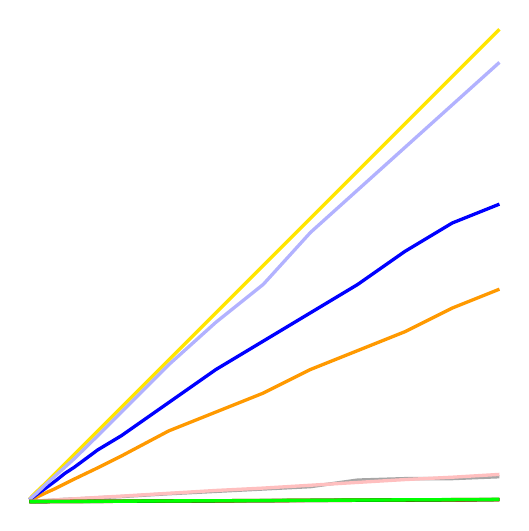
\begin{tikzpicture}[xscale=0.6,yscale=0.6]
		\DrawAxes{steps}{time~(sec)}
		\GridOn
		\TicksOn
		\XAxisText{0.05cm/25}{1cm/}{2cm/1000}{3cm/}{4cm/2000}{5cm/}{6cm/3000}{7cm/}{8cm/4000}
		\XAxisText{9cm/}{10cm/5000}{}{}{}{}{}{}{}
		\YAxisText{0.00cm/0}{1.00cm/280}{2.00cm/560}{3.00cm/840}{4.00cm/1120}{5.00cm/1400}{6.00cm/1680}{7.00cm/1960}{8.00cm/2240}
		\YAxisText{9.00cm/2520}{10.00cm/2800}{}{}{}{}{}{}{}
		% ------- 2D temporal with 512^2 size -------
		\draw[line width=1.2pt,color=red!40!yellow] (0.05cm,0.027cm) -- (0.1cm,0.047cm) -- (0.2cm,0.094cm) -- (0.4cm,0.19cm) -- (0.6cm,0.28cm) -- (0.8cm,0.38cm) -- ( 1cm,0.48cm) -- (1.5cm,0.72cm) -- ( 2cm,0.97cm) -- ( 3cm,1.5cm) -- ( 4cm,1.9cm) -- ( 5cm,2.3cm) -- ( 6cm,2.8cm) -- ( 7cm,3.2cm) -- ( 8cm,3.6cm) -- ( 9cm,4.1cm) -- (10cm,4.5cm);
		\draw[line width=1.2pt,color=red!10!yellow] (0.05cm,0.052cm) -- (0.1cm,0.11cm) -- (0.2cm,0.21cm) -- (0.4cm,0.4cm) -- (0.6cm,0.6cm) -- (0.8cm,0.8cm) -- ( 1cm, 1cm) -- (1.5cm,1.5cm) -- ( 2cm, 2cm) -- ( 3cm, 3cm) -- ( 4cm, 4cm) -- ( 5cm, 5cm) -- ( 6cm, 6cm) -- ( 7cm, 7cm) -- ( 8cm, 8cm) -- ( 9cm, 9cm) -- (10cm,10cm);
		\draw[line width=1.2pt,color=blue] (0.05cm,0.046cm) -- (0.1cm,0.076cm) -- (0.2cm,0.15cm) -- (0.4cm,0.29cm) -- (0.6cm,0.44cm) -- (0.8cm,0.6cm) -- ( 1cm,0.73cm) -- (1.5cm,1.1cm) -- ( 2cm,1.4cm) -- ( 3cm,2.1cm) -- ( 4cm,2.8cm) -- ( 5cm,3.4cm) -- ( 6cm, 4cm) -- ( 7cm,4.6cm) -- ( 8cm,5.3cm) -- ( 9cm,5.9cm) -- (10cm,6.3cm);
		\draw[line width=1.2pt,color=blue!30!white] (0.05cm,0.048cm) -- (0.1cm,0.094cm) -- (0.2cm,0.18cm) -- (0.4cm,0.37cm) -- (0.6cm,0.55cm) -- (0.8cm,0.73cm) -- ( 1cm,0.91cm) -- (1.5cm,1.4cm) -- ( 2cm,1.9cm) -- ( 3cm,2.9cm) -- ( 4cm,3.8cm) -- ( 5cm,4.6cm) -- ( 6cm,5.7cm) -- ( 7cm,6.6cm) -- ( 8cm,7.5cm) -- ( 9cm,8.4cm) -- (10cm,9.3cm);
		\draw[line width=1.2pt,color=gray!70!white] (0.05cm,0.014cm) -- (0.1cm,0.01cm) -- (0.2cm,0.016cm) -- (0.4cm,0.026cm) -- (0.6cm,0.038cm) -- (0.8cm,0.053cm) -- ( 1cm,0.059cm) -- (1.5cm,0.086cm) -- ( 2cm,0.11cm) -- ( 3cm,0.17cm) -- ( 4cm,0.22cm) -- ( 5cm,0.27cm) -- ( 6cm,0.32cm) -- ( 7cm,0.46cm) -- ( 8cm,0.49cm) -- ( 9cm,0.49cm) -- (10cm,0.53cm);
		\draw[line width=1.2pt,color=pink] (0.05cm,0.0099cm) -- (0.1cm,0.011cm) -- (0.2cm,0.017cm) -- (0.4cm,0.028cm) -- (0.6cm,0.04cm) -- (0.8cm,0.051cm) -- ( 1cm,0.063cm) -- (1.5cm,0.092cm) -- ( 2cm,0.12cm) -- ( 3cm,0.18cm) -- ( 4cm,0.24cm) -- ( 5cm,0.29cm) -- ( 6cm,0.35cm) -- ( 7cm,0.41cm) -- ( 8cm,0.47cm) -- ( 9cm,0.52cm) -- (10cm,0.58cm);
		\draw[line width=1.2pt,color=red!70!black] (0.05cm,0.003cm) -- (0.1cm,0.0025cm) -- (0.2cm,0.0029cm) -- (0.4cm,0.0037cm) -- (0.6cm,0.0045cm) -- (0.8cm,0.0053cm) -- ( 1cm,0.0062cm) -- (1.5cm,0.0082cm) -- ( 2cm,0.01cm) -- ( 3cm,0.015cm) -- ( 4cm,0.018cm) -- ( 5cm,0.023cm) -- ( 6cm,0.027cm) -- ( 7cm,0.031cm) -- ( 8cm,0.035cm) -- ( 9cm,0.039cm) -- (10cm,0.043cm);
		\draw[line width=1.2pt,color=red] (0.05cm,0.0068cm) -- (0.1cm,0.0041cm) -- (0.2cm,0.0045cm) -- (0.4cm,0.0054cm) -- (0.6cm,0.0063cm) -- (0.8cm,0.0072cm) -- ( 1cm,0.0083cm) -- (1.5cm,0.011cm) -- ( 2cm,0.013cm) -- ( 3cm,0.017cm) -- ( 4cm,0.022cm) -- ( 5cm,0.027cm) -- ( 6cm,0.031cm) -- ( 7cm,0.036cm) -- ( 8cm,0.04cm) -- ( 9cm,0.045cm) -- (10cm,0.05cm);
		\draw[line width=1.2pt,color=green!50!black] (0.05cm,0.0029cm) -- (0.1cm,0.0026cm) -- (0.2cm,0.0031cm) -- (0.4cm,0.0039cm) -- (0.6cm,0.0048cm) -- (0.8cm,0.0057cm) -- ( 1cm,0.0066cm) -- (1.5cm,0.0088cm) -- ( 2cm,0.011cm) -- ( 3cm,0.016cm) -- ( 4cm,0.02cm) -- ( 5cm,0.024cm) -- ( 6cm,0.029cm) -- ( 7cm,0.033cm) -- ( 8cm,0.038cm) -- ( 9cm,0.042cm) -- (10cm,0.047cm);
		\draw[line width=1.2pt,color=green] (0.05cm,0.0045cm) -- (0.1cm,0.0036cm) -- (0.2cm,0.0041cm) -- (0.4cm,0.0051cm) -- (0.6cm,0.006cm) -- (0.8cm,0.0072cm) -- ( 1cm,0.0079cm) -- (1.5cm,0.01cm) -- ( 2cm,0.013cm) -- ( 3cm,0.018cm) -- ( 4cm,0.022cm) -- ( 5cm,0.027cm) -- ( 6cm,0.032cm) -- ( 7cm,0.036cm) -- ( 8cm,0.041cm) -- ( 9cm,0.046cm) -- (10cm,0.051cm);
	\end{tikzpicture}
\label{fig:Peformance-comparison:Temporal}
\end{figure}
\end{frame}
\begin{frame}{Performance Analysis: Legend}
\begin{figure}[H]
\vspace{-0.5cm}
\centering
\begin{tikzpicture}
\DrawLegend
\end{tikzpicture}
\label{fig:Peformance-comparison:legend}
\end{figure}
\end{frame}
\section{FDTD Modelling of Cylindrical Cloak}
\begin{frame}{FDTD Modelling of Cylindrical Cloak}
	\begin{itemize}
	\item Intro
	\item Geometry
	\end{itemize}
\end{frame}

\section{Conclusion}
\begin{frame}{Conclusion}
	\begin{itemize}
	\item Speed--up of 10x--20x
	\end{itemize}
\end{frame}

\section{References}
\begin{frame}[t,allowframebreaks]{References}
	\nocite{*}
	\bibliographystyle{ieeetr} %plain, ieeetr
	{\tiny \bibliography{FDTDref}}
\end{frame}
\end{document}